\documentclass[a4paper]{article}
\usepackage[utf8]{inputenc}
\usepackage[T1]{fontenc}
\usepackage{graphicx}
\usepackage{longtable}
\usepackage{hyperref}
\usepackage{caption}

\usepackage[margin=1.5in]{geometry}
\usepackage{setspace}
\onehalfspacing

\usepackage{fancyhdr}
\pagestyle{fancy}
\fancyhead{}
\fancyfoot{}
\fancyhead[LE,RO]{\leftmark}
\fancyhead[RE,LO]{Niklas Reinhold}
\fancyfoot[C]{\thepage}
\renewcommand{\headrulewidth}{0.4pt}
\renewcommand{\footrulewidth}{0pt}

\usepackage[backend=biber, style=numeric]{biblatex}
\addbibresource{./references.bib}

\usepackage[numbib,notlof,notlot,nottoc]{tocbibind}
\pagenumbering{gobble}

\begin{document}
	
\begin{titlepage}

    \newcommand{\HRule}{\rule{\linewidth}{0.1mm}} % Defines a new command for the horizontal lines, change thickness here

    \center % Center everything on the page
	
   \textsc{\Large Master Thesis Proposal}\\[0.5cm] % Major heading such as course name
	    
    %----------------------------------------------------------------------------------------
    %	TITLE SECTION
    %----------------------------------------------------------------------------------------
    
    \HRule \\[0.4cm]
    { \huge \bfseries Open Blockchain-based Local Energy Market Simulation Platform}\\[0.7cm] % Title of your document
    \HRule \\[0.4cm]
    
    \vspace{2cm}

    %----------------------------------------------------------------------------------------
    %	INSTITUTION SECTION
    %----------------------------------------------------------------------------------------
    
    % LOGO 
    
\includegraphics[width=0.15\textwidth]{img/uni_cologne.png}\\[1cm] % Include a department/university logo - this will require the graphicx package
    
   \textsc{\LARGE University of Cologne}\\[0.5cm] % Name of your university/college
   
   % DEPARTMENT
    \large
    Department of Information Systems for Sustainable Society\\
    Faculty of Management, Economics and Social Sciences\\
   
	\vspace{3cm}
	
    %----------------------------------------------------------------------------------------
    %	AUTHOR SECTION
    %----------------------------------------------------------------------------------------
    
	\large
	\textbf{Author}: Niklas Reinhold\\
	\large
	\textbf{Supervisor}: Prof. Dr. Wolfgang Ketter
	
	\vspace{2cm}

    %----------------------------------------------------------------------------------------
    %	DATE SECTION
    %----------------------------------------------------------------------------------------

    {\large \today}\\[1cm] % Date, change the \today to a set date if you want to be precise

    \vfill  % Fill the rest of the page with whitespace
    

\end{titlepage}


\pagenumbering{Roman}
\tableofcontents
\clearpage
\listoffigures
\clearpage
%\listoftables
%\clearpage

\pagenumbering{arabic}

\section{Research Motivation}
\label{sec:research_motivation}
\section{Introduction}
Global warming is one of the most crucial challenges of our time. A shift 
to sustainable energy sources is needed, which necessitates the cooperation of several disciplines. 
However, the integration of \textit{renewable energy sources (RES)} into the existing grid is 
a complex issue and requires new market approaches. 
This thesis follows the idea of \textit{local energy markets (LEM)} and combines the themes of 
distributed resource optimization and the emerging \textit{distributed ledger technology (DLT)} 
to develop a platform for simulating blockchain-based \textit{local energy markets (LEM)}.


\subsection{Research Motivation}
\label{sec:research_motivation}

% RES, explanation and so
The generation from distributed RES is constantly increasing \shortcite{mengelkamp2018designing}. 
In contrast to power plants which run by non-renewable fossil fuels, distributed RES produce energy in a decentralized and volatile way, which is hard to predict. 
These characteristics of the distributed RES challenge the current energy system \shortcite{ampatzis2014local}.
% the current electric grid and the problems
The existing electric grid is built for centralized generation by large power plants 
and the design of the current wholesale markets
is not able to react in real-time to a significant amount of distributed RES \shortcite{mengelkamp2018designing}. 
Moreover, this way of energy generation is economically not ideal because of energy losses due to long physical
distances between generation and consumption parties. 
% introduction of p2p energy trading
Therefore, new market approaches are needed, to successfully integrate the increasing amount of distributed RES \shortcite{mengelkamp2018blockchain}. 
A possible solution to the technical and market problems is \textit{peer-to-peer (P2P)} energy trading in LEM \shortcite{long2017feasibility}. 
% explanation of local energy markets
LEM, also called microgrid energy markets, consist of small scale prosumers, consumers and a market platform that enables the trading 
of locally generated energy between the parties of a community.
Due to the trading of locally generated energy within the related communities,
LEM support sustainability and the efficient use of distributed RES.
Likewise, the need for expensive and inefficient transportation of energy through long physical 
distances can be reduced. The concept of LEM strengthens the self-sufficiency of communities and 
enables possible energy cost reductions. Moreover, profits remain within the communities 
by which reinvestments in additional RES are promoted \shortcite{mengelkamp2018designing}. 

% introduction of blockchain as underlying technology 
However, P2P energy trading in LEM requires advanced communication and data exchanges between the different parties, 
which makes central management and operation more and more challenging. The implementation of LEM need local 
distributed control and management techniques \shortcite{andoni2019blockchain}. 
Therefore, a new and innovative \textit{information communication technology (ICT)} is required.  
The emerging DLT provides a possible solution. 
It is designed to enable distributed transactions without a central trusted entity. 
A blockchain allows the automated execution of smart contracts depending 
on vesting conditions, which suits the need of LEM for decentralized and autonomous market mechanisms. 
This offers new approaches and market designs. Accordingly, DLT can help to address the challenges 
faced by decentralized energy systems. However, DLTs are not a mature technology yet and 
there are several barriers in using them, especially for the researcher who do not have a technical background. 

% introduce the topic of competitive benchmarking
Due to the plurality of involved parties and the interdisciplinary requirements for the 
implementation of new energy market approaches, the accessibility is of major importance.
\shortciteA{ketter2015competitive} introduce the approach of \textit{Competitive Benchmarking (CB)}. 
This approach describes a research method that faces a real-world wicked problem that is beyond the capacity of a single discipline. 
It is realized by developing a shared paradigm that is represented in a concrete open simulation platform. 
In detail, it consists of the three principal elements \textit{CB Alignment}, \textit{CB Platform} and \textit{CB Process}. 
The CB Alignment refers to the constant synchronization process between the shared paradigm and the wicked problem. 
The CB Platform represents the medium in which the shared paradigm is technically illustrated
and provides the infrastructure for the third element CB Process. 
It describes the iterative development of new theories and design artifacts through independent researchers, 
who influence each other and improve their work in direct sight of each other.
The presence of such an open simulation platform depicting the shared paradigm of LEM, 
would ensure the accessibility and could help to gain new valuable outcomes in the research field 
of LEM or new energy market designs in general.

% introduction of optimization decomposition algorithm
Further, the welfare optimization of all participants in LEM can be represented by the 
central problem of the \textit{Bundle Trading Market Framework (BTM)} developed by \shortciteA{guo2007market}.
It constitutes a market-based optimization algorithm
that solves a distributed system optimization problem by self-interested agents iteratively 
trading bundled resources in a double auction market run by a dealer.
The dealer maximizes the welfare through allowing agents 
to trade their preferred bundles of energy. Hence, the stated BTM implemented on the basis of a 
blockchain as underlying ICT can represent the concept of LEM.
% bringing all together

This research brings all the introduced approaches together 
and develops an open \textit{blockchain-based LEM Simulation (BLEMS)}, which enables the research 
approach based on the three stated elements of CB. The BLEMS is realized through 
the introduced optimization algorithm with a blockchain as the underlying ICT. 
That means, the smart contract takes the role of the market dealer and the self-interested 
agents represent the individual participants. This paper focuses on the 
implementation and software design of the open BLEMS.

\clearpage

\section{Literature Review}
\label{sec:literature_review}
\section{Literature Review}
\label{sec:literature_review}

\subsection{Blockchain-based Energy Markets}
\label{sec:Blockchain-based Energy Markets}
To start, \shortciteA{mihaylov2014nrgcoin} were the first who addressed blockchain technology in
energy markets. They presented a new decentralized digital currency with the aid of
which prosumers can trade locally produced renewable energy.
In their introduced concept, the generation and consumption of renewable energy are directly
transferable into virtual coins. However, the market value of the virtual currency is determined
centrally by the distributed system operator. Further, \shortciteA{al2015bitcoin} introduced a blockchain-based
model for a decentralized carbon emission trading infrastructure.
Their model based on the bitcoin protocol and focus on privacy and system security goals.
Besides, they provide a solution to the problem of anonymous carbon emission trading.
Equally, \shortciteA{aitzhan2018security} addressed the issue of transaction security in
decentralized smart grid energy trading and implemented a proof-of-concept for a
blockchain-based energy trading system including anonymous encrypted messaging streams.
Concluding, they have shown that blockchains enable the implementation of decentralized energy trading and that the degree
of privacy and security is higher than in traditional centralized trading platforms. 
Furthermore, \shortciteA{sikorski2017blockchain}
presented a proof-of-concept where a blockchain enables machine-to-machine (M2M) interactions depicting an
M2M energy market. They pointed out that the blockchain technology has
significant potential to support and enhance the 4th industrial revolution. 
Moreover, \shortciteA{mengelkamp2018designing}
revealed the concept of a blockchain-based local energy market without the need of a thrusted
third entity. In addition, they deduced seven market
components as a framework for building efficient microgrid energy markets. Consequently,
the Brooklyn Microgrid project is introduced and evaluated according to the market components.
As a result, the Brooklyn Microgrid has also shown that blockchains are a suitable technology
to implement decentralized microgrid energy markets, though current regulation does not
allow running such LEM in most of the countries. Later on, \shortciteA{mengelkamp2018blockchain}
presented a initial proof-of-concept of a simple blockchain-based concept, market design and
simulation of a local energy market consisting of a hundred households.
Finally, they concluded that the real-life realization and technological limitations of such blockchain-based
market approaches need to be investigated by further research. 
In addition, it is mentioned that regulatory
changes will play an important role in the future of blockchain-based LEM.

\subsection{Distributed Resource Optimization}
\label{sec:Distributed Resource Optimization}
To begin with, \shortciteA{fan2003decentralized} outlined a new approach for the 
development of an information system
that can be used for the problem of a supply chain. The concept demonstrated a decentralized
decision-making process that is realized through the design of a market-based coordination
system which incites the participants to act in a way that is beneficial to the overall
systems. Further, \shortciteA{guo2007market} revived this concept
and developed the BTM, a market-based decomposition method for decomposable linear systems,
which can be easily implemented to support real-time optimization of distributed
systems. They proved that the system optimality can be
achieved under a dynamic market-trading algorithm in a finite number of trades.
Moreover, the outlined algorithm can be operated in synchronous and as well in
asynchronous environments. Later on, \shortciteA{guo2012computational} extended 
their stated concept to a dynamic, asynchronous internet market environment.
Additionally, they examined how various market design factors like dealer inventory
policies, market communication patterns, and agent learning strategies affect
computational market efficiency and implementation. Finally,
they proved finite convergence to an optimal solution under all these different schemes.

\subsection{Competitive Benchmarking}
Firstly, \shortciteA{march1995design} described a two-dimensional framework for research in IS.
The two dimensions can be distinguished into behavioral-science and design-science. The behavioral-science
paradigm is based on explaining and predicting human or organizational behavior. Whereas, the design-science
paradigm is based on broad types of outputs produced by design research. It strives to extend the boundaries
of human and organizational capabilities through the creation of new artifacts.

% connection of these two - design science approach by hevner
Furthermore, the research framework presented by \shortciteA{hevner2008design} combines both stated
IT research paradigms and illustrates the interaction between these two.
They presented that technology and behavior are inseparable in an information system. Therefore,
they argued that considering the complementary research cycle between design-science and behavioral-science
is crucial to address fundamental problems faced in the productive application of information technology.

% competitive benchmarking include basic principles of hevner
In addition, \shortciteA{ketter2015competitive} introduced the IS research approach CB,
which includes various basic principles of the design science approach of \shortciteA{hevner2008design}.
This IS research concept is designed for so-called wicked problems and addresses the problems and needs of interdisciplinary
research communities. CB focuses on the interconnection of problems at the same and different levels to imitate the real world.
In repeated competitions, in which individual teams compete against each other, the developed environment and models
can be tested and evaluated. This results in a diversity of outcoming designs, which are difficult to achieve in
traditional design science frameworks.

\clearpage
\clearpage

\section{Research Design}
\label{sec:research_design}
\section{Research Design}
\label{sec:research_design}

This research is inspired by the stated CB research approach and focus on the development of 
the second CB element, an open simulation platform depicting the shared paradigm of a LEM. 
The proposed design is presented in Figure \ref{figure:competitive_benchmarking}. 
In contrast to the inital CB research design, the third element \textit{CB Process} differs. 
The paltform enables research groups to design and test their artifacts in the field of the shared 
paradigm, using the developed platform. However, the designed artifacts in the form of autonomous 
software agents do not compete against each other in competitions. 
Rather, research groups are able to design and develop the behavior of all agents and the 
autonomous market mechanism. Hence, it is also possible to analyze and evaluate the designed 
artifacts and use them as a benchmark to compare different designs. 

\begin{figure}[htbp]
	\centering
	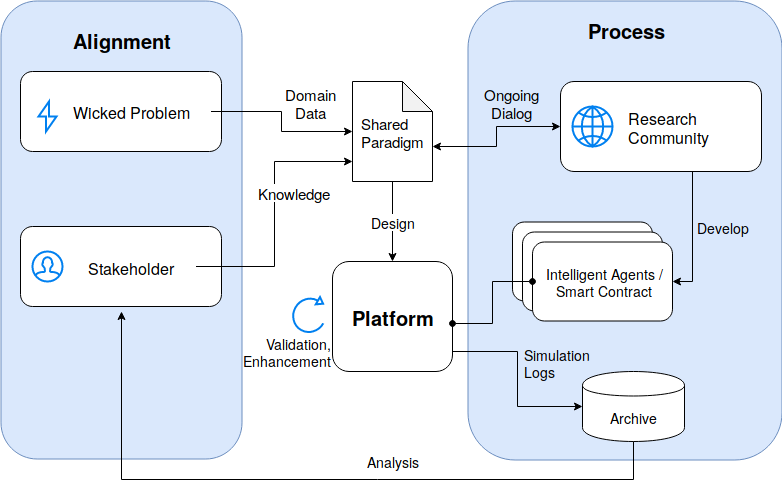
\includegraphics[width=1\linewidth]{./figures/competitive_benchmarking.png}
	\caption{Research Design following \protect\shortciteA{ketter2015competitive}}
	\label{figure:competitive_benchmarking}
\end{figure}

According to the IS Design Science principles introduced by Hevner, March, Park, and Ram \shortcite{hevner2008design}, 
the presented research design produce a viable artifact in the form of an open simulation platform, which depict a 
relevant real-world wicked problem. Due to the outcoming data produced by the simulation platform, 
it is possible to develop methods to evaluate the utility, quality and efficacy of the artifact. 
Moreover, the research provide a varifable contribution through the artifact, the open simulation platform, itself. 
The platform enables the investigation of possible solutions of unsolved problems and further, 
it removes the technical barriers for the use of the complex distributed ledger technology. 
Besides, the implementation of the platform is based on an appropriate selection of techniques. 
As stated in \ref{sec:Blockchain-based Energy Markets}, 
blockchains are a suitable technology to implement decentralized microgrid energy markets. 
In addition, the in \ref{sec:Distributed Resource Optimization} introduced distributed optimization 
algorithm achieve evidentially system optimality under a dynamic market-trading algorithm. 
Therefore, this research relies upon the application of rigorous methods and comply the requirement 
of the fifth guideline by \shortciteA{hevner2008design}. 
In addition, the platform enables the iterative search for an optimal design through the comparison 
of different produced solutions and is valuable to technology-oriented as well as management-oriented 
audiences. As a result, these research design also fulfil the seven research guidlines of 
the research framework introduced by \shortciteA{hevner2008design}. 


\section{Expected Contribution}
\label{sec:expected_contribution}
\section{Expected Contribution}
\label{sec:expected_contribution}

This research provides two different contributions. First, the fully decentralization of the introduced distributed optimization algorithm \shortcite{guo2007market}. 
The bundle-trading market grant access of any given trade to the market dealer. This, again, necessitates trust of the agents that it will use those resources according to the over-arching organizational goal. Due to the implementation of the market dealer by a smart contract, the technical implementation is public accesible. Moreover, all transactions of the market dealer to allocate the resources are transparent. Therefore, the behavior of the market dealer is comprehensible for every participant. Furthermore, it provides a high degree of security due to cryptographic encryption methods which are essential parts of the blockchain.
Second, the open simulation platform itself. From the scientific perspective, the platform is relevant due to the removal of existing technical barriers for practicioners in using complex distributed ledgers technologies. Therefore the platform facilitates researchers without a deep technically background to use those DLTs and incentivises to design and test their artifacts by using this platform. 
On the other hand, from a business perspective, this research is relevant to policy makers and energy suppliers. The platform allows stakeholders to get a better understanding of the dynamics of decentralized LEM and enables the testing and evaluating of policy options and implications. 

\clearpage
\clearpage

\section{Simulation Platform Architecture}
\label{sec:Simulation Platform Architecture}
This chapter gives a short representation of the first platform design and the chosen technologies and frameworks. First, the Ethereum blockchain is implemented through Ganache. It is a personal local blockchain for the Ethereum development, which can be used to deploy smart contracts, develop decentralized applications, and run tests. Further, Ganache is available as a desktop application as well as a command-line tool. Next, the role of the market dealer is realized by a smart contract which is written in Solidity. This object-oriented programming language was especially designed for developing smart contracts that run on a Ethereum blockchain. The Solidity code is compiled to bytecode, which can be deployed into the blockchain. Moreover, the clients which constitute the different agents are implemented through the programming language Python. Python is a object oriented, high-level programming  language with a easy and simple to learn syntax. Therefore, the hurdles in modifying the client behavior are minimized. Finally, the clients using the Web3.py python library for the interaction with the Ethereum blockchain. 

\begin{figure}[htbp]
	\centering
	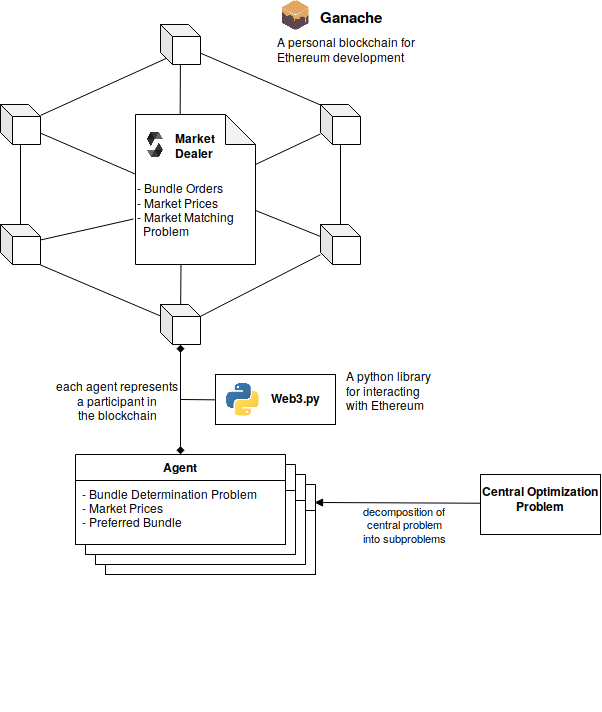
\includegraphics[width=.8\linewidth]{./figures/platform_architecture.png}
	\caption{Platform Design}
	\label{figure:paltform_architecture}
\end{figure}

\clearpage
\printbibliography

\end{document}
